\documentclass{article}

\input{../../base}
\input{../../cmds}
\input{../../format}
\input{../course}

\usepackage{caption}
\usepackage{subcaption}
\usepackage{tikz}
\usetikzlibrary{shapes.geometric}
\usepackage{tikz-3dplot}
\usepackage{setspace}

\newcommand{\ngon}[1]{%
    \begin{tikzpicture}
        \node[draw,regular polygon,regular polygon sides=#1,minimum size=3cm] (a) {};
        \foreach \k in {1,2,...,#1} {\draw (a.center) -- (a.corner \k);}
    \end{tikzpicture}
}

\newcommand{\ngoncyl}[1]{%
    \tdplotsetmaincoords{70}{110}
    \begin{tikzpicture}[tdplot_main_coords]
        \def\r{1}
        \def\h{2.616}
        \node[fill,inner sep=0cm] (a) at (0, 0, 0) {};
        \node[fill,inner sep=0cm] (b) at (0, 0, \h) {};
        \foreach \k in {1,2,...,#1} {
            \tdplotsinandcos{\sintheta}{\costheta}{\k*360/#1}
            \node[fill,inner sep=0cm] (a\k) at (\costheta,\sintheta,0) {};
            \node[fill,inner sep=0cm] (b\k) at (\costheta,\sintheta,\h) {};
            \draw (a) -- (a\k) -- (b\k) -- (b);
        }
        \foreach \k in {2,3,...,#1} {
            \pgfmathsetmacro{\lastk}{\k-1}
            \draw (a\lastk) -- (a\k) -- (b\lastk) -- (b\k);
        }
        \draw (a#1) -- (a1) -- (b#1) -- (b1);
    \end{tikzpicture}
}

\begin{document}

\makeheader{Heimadæmi 1}

\section*{Dæmi 1}
Athuga á hvernig hægt væri að skilreina fylltan sívalning eingöngu með
þríhyrningum í þrívíðu rúmi.

\smallskip\par\textbf{Svar:}
Byrjum fyrst að skoða hvernig hægt væri að skilgreina flata hringskífu
með þríhyrningum. Það má gera með að nálga hringskífuna með reglulegum 
marghyrningi, en auðvelt er að skilgreina $n$-hliða marghyrning með
þríhyrningum með því að velja einn punkt $a$ innaní marghyrningnum og 
búa so til $n$ þríhyrninga, hver með einn hornpunkt í $a$ og mótliggjandi
hlið í einhverri hlið marghyrningsins (þannig að engir tveir þríhyrningar
deili marghyrningshlið sinni).
Í tilvikinu þegar marghyrningurinn er reglulegur er eðlilegt að
velja $a$ sem miðpunkt hans. Svona nálgun á hringskífu má sjá að neðan
fyrir mismunandi gildi á $n$.

\begin{figure}[h!]
    \centering
    \begin{subfigure}[b]{0.3\textwidth}
        \centering
        \ngon{10}
        \caption*{$n=10$}
    \end{subfigure}
    \begin{subfigure}[b]{0.3\textwidth}
        \centering
        \ngon{20}
        \caption*{$n=25$}
    \end{subfigure}
    \begin{subfigure}[b]{0.3\textwidth}
        \centering
        \ngon{33}
        \caption*{$n=40$}
    \end{subfigure}
\end{figure}

Við sjáum að sannfærandi niðurstaða fæst þegar valið er $n=40$.

Nú má búa til sívalning með tveimur slíkum marghyrningum með því
að raða þeim þannig að einn fáist frá öðrum með því að hliðra honum
um einhverja vegalengd samsíða þverás hans, og tengja saman hverja hlið
eins marghyrningsins við samsvarandi hlið hins með rétthyrningum
sem búnir eru til úr tveimur þríhyrningum eins og að neðan.

\begin{figure}[h!]
    \centering
    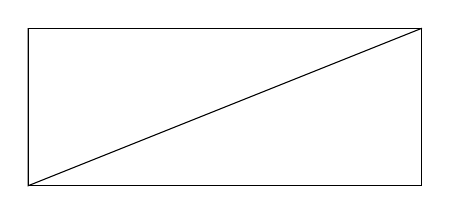
\begin{tikzpicture}[scale=0.5]
        \draw (-5, 2) -- (5, 2) -- (5, -2) -- (-5, -2);
        \draw (-5, 2) -- (-5, -2) -- (5, 2);
    \end{tikzpicture}
\end{figure}

Lokaniðurstöðuna má nú sjá að neðan.
\begin{figure}[h!]
    \centering
    \begin{subfigure}[b]{0.3\textwidth}
        \centering
        \ngoncyl{10}
        \caption*{$n=10$}
    \end{subfigure}
    \begin{subfigure}[b]{0.3\textwidth}
        \centering
        \ngoncyl{25}
        \caption*{$n=25$}
    \end{subfigure}
    \begin{subfigure}[b]{0.3\textwidth}
        \centering
        \ngoncyl{40}
        \caption*{$n=40$}
    \end{subfigure}
\end{figure}

Athugum að fyrir hverja hlið marghyrninganna eru notaðir
fjórir þríhyrningar í sívalningnum (einn í hvorri skífu
og tveir í möttli sívalningsins).
Fjöldi þríhyrninga sem notaðir eru fyrir sívalninginn er því $4n$,
sér í lagi eru $100$ þríhyrningar notaðir fyrir $n=25$
og $160$ notaðir fyrir $n=40$
Sannfærandi þríhyrningur notar þá a.m.k.~hundrað þríhyrninga, jafnvel fleiri.

\section*{Dæmi 2}
Gera á grein fyrir innri bandvídd, litahraða skjápunkta, ytri bandvídd og
hámarks skjáupplausn og sjónvarps/skjá staðal grafíkkortsins Nvidia GeForce
RTX 3090.

\smallskip\par\textbf{Svar:}
\begin{itemize}
        \item Innri bandvíddin er 936 GB/s.
        \item Litahraði skjápunkta er $156{,}2$ GP/s, þ.e. $156{,}2$
        milljarðir skjápunkta á sekúndu.
        \item Ytri bandvíddin er 384 GB/s.
        \item Hámarks skjáupplausnin er 7680x4320 með staðlinum HDMI 2.1.
\end{itemize}

\section*{Dæmi 3}
Gera á grein fyrir sumum af kostum grafíkforritasafnsins Vulkan yfir OpenGL.

\smallskip\par\textbf{Svar:}
Meginkostur Vulkan yfir OpenGL er betri nýting örgjörvans og grafíkkortsins.
Vulkan gefur forriturum einnig meiri stjórn yfir grafíkkortið.
Ásamt þessu er Vulkan auðflytjanlegt á milli stýrikerfa og notar
sama API fyrir borð- og smátölvur, ólíkt OpenGL.

Vulkan er hraðvirkara en OpenGL en það eru enn kostir við OpenGL.
Oft er ekki þörf fyrir hið öflugsta og í þeim tilvikum er OpenGL
góður valmögleiki, en það er erfiðara að forrita með Vulkan þar sem
það er lægra sett en OpenGL.

\section*{Dæmi 4}
Gera á grein fyrir tilgangi opnu staðlana glTF og OpenXR.

\smallskip\par\textbf{Svar:}
Staðallinn glTF er ætlaður til að geyma gögn um þrívíð líkön á hagstæðan hátt.
Gögn sem fylgja þessum staðli eru geymd í skrám með nafnauka \verb|.gltf| eða \verb|.glb|

Staðallinn OpenXR er notaður fyrir samskipti tölva og sýndar- og viðvótarveruleikatækja.
Hann gefur forriturum staðlaðann API til þessa tilgangs.

\newpage

\section*{Dæmi 5}
Keyra á þéttilista Sierpinskis með auknum fjölda punkta.

\smallskip\par\textbf{Keyrsla:}
Keyrsluna má sjá í skjáskoti að neðan.

\begin{figure}[!h]
    \centering
    \includegraphics[width=\textwidth]{keyrsla}
\end{figure}

Hér á eftir má sjá útgafu forritsins skrifaða með forritunarmálinu Elm
ásamt WebGL pakka.

{\setstretch{1.0}\footnotesize\begin{verbatim}
module Main exposing (main)

import Browser
import Html exposing (Html)
import Html.Attributes exposing (height, style, width)
import Random
import WebGL exposing (Mesh, Shader)
import Math.Vector2 exposing (Vec2, vec2, add, scale, getX, getY)
import Math.Vector4 exposing (Vec4, vec4)

numPoints : Int
numPoints = 50000

-- MAIN --

-- Forritið í heild sinni.
main : Program () (Mesh Vertex) Msg
main = Browser.element
    { init = init
    , update = update
    , view = view 
    , subscriptions = \_ -> Sub.none
    }



-- INIT --

-- Fall sem er kallað á þegar forritið er fyrst keyrt.
-- Í þessu tilviki sendir það skilaboð á keyrsluumhverfið
-- að búa til nýtt mesh. Keyrsluumhverfið beinir þessu
-- á update fallið.
init : () -> (Mesh Vertex, Cmd Msg)
init _ =
    ( WebGL.points []
    , Random.generate NewMesh <| points numPoints
    )

--< Mesh >--

-- Hornpunktar þríhyrningsins
v0 = vec2 -1 -1
v1 = vec2  0  1
v2 = vec2  1 -1

-- Fall til að bæta nýjum punkti við punktalistann
-- fyrir gefið horn sem á að færa síðasta punktinn að.
-- Notað sem hjálparfall í points.
addNextPoint : Vec2 -> List Vec2 -> List Vec2
addNextPoint corner prev =
    case List.head prev of
        Nothing -> []
        Just p -> (scale 0.5 <| add corner p) :: prev

-- Fall sem skilar leið til þess að framleiða
-- slembinn lista af punktum innan þríhyrningsins.
-- Þar sem Elm er hreint (pure) forritunamál
-- getur þetta fall ekki einfaldega skilað lista af
-- punktum eins og t.d. í JavaScript.
points : Int -> Random.Generator (List Vec2)
points n =
    let corners = Random.list n <| Random.uniform v0 [v1, v2]
        u = add v0 v1
        v = add v0 v2
        p = scale 0.25 <| add u v
    in  Random.map (List.foldl addNextPoint [p] >> List.reverse) corners



-- UPDATE --

-- Skilaboð sem keyrsluumhverfið fær.
-- Í þessu tilviki er eina skilaboðið
-- það að búa til nýtt mesh að gefnum
-- lista af punktum.
type Msg = NewMesh (List Vec2)

-- Fall sem tekur skilaboð og núverandi ástand
-- kerfisins og skilar nýju kerfi ásamt
-- skipun til keyrsluumhversins.
update : Msg -> Mesh Vertex -> (Mesh Vertex, Cmd Msg)
update (NewMesh vs) _ =
    ( WebGL.points <| List.map makeVertex vs
    , Cmd.none
    )

-- Fall til að búa til Vertex úr tvívíðum vigri
-- (sjá skilgreiningu á Vertex að neðan).
-- Þetta þarf þar sem Elm styður ekki að
-- senda tvívíðan vigur inn í fjórvítt attribute
-- eins og hægt er að gera í JavaScript (og er
-- gert í JavaScript-útgáfu þessa forrits).
makeVertex : Vec2 -> Vertex
makeVertex v = { vPosition = vec4 (getX v) (getY v) 0 1 }



-- VIEW --

-- Tagið Vertex er notað til að tala við
-- hnútalitarann og inniheldur öll attribute
-- sem notuð eru í honum, með sama nafn og
-- sama tag.
type alias Vertex = { vPosition : Vec4 }

-- View fallið tekur núverandi ástand kerfisins
-- og skilar HTML-kóða til að birta.
view : Mesh Vertex -> Html Msg
view mesh =
    WebGL.toHtml 
        [ width 512
        , height 512 
        ] 
        [ WebGL.entity 
            vertexShader
            fragmentShader
            mesh
            {}
        ]

--< Shaders >--

-- Litarar skrifaðir með venjulegum GLSL-kóða.

vertexShader : Shader Vertex {} {}
vertexShader = [glsl|

attribute vec4 vPosition;

void main() {
    gl_PointSize = 1.0;
    gl_Position = vPosition;
}

|]

fragmentShader : Shader {} {} {}
fragmentShader = [glsl|

precision mediump float;

void main() {
    gl_FragColor = vec4(1.0, 0.0, 0.0, 1.0);
}

|]
\end{verbatim}}

Útkoma þessa forrits er jafngild því að ofan eins og sjá má að skjáskoti á næstu síðu.
Elm þýðist yfir í eina (mjög) stóra HTML (eða JavaScript) skrá og má
lok hennar sjá til hægri á skjáskotinu. 

Ég skrifaði þessa útgáfu aðallega til þess að æfa mig í Elm og
til þess að fá lyktina af því hvernig þessi pakki virkar.
Eins og sést að ofan er þetta töluvert hærra sett (high-level)
en venjulegi API-inn í JavaScript.
Ég myndi vel skilja ef þú ákveður að leyfa ekki að skila með Elm,
en ef þú ákveður annað myndi ég vilja halda áfram að því.

\begin{figure}[!ht]
    \centering
    \includegraphics[width=\textwidth]{elm-keyrsla}
\end{figure}

\end{document}
